\section{Introduction}\label{sec:intro}

Nowhere dense classes of graphs were introduced 
by Ne\v set\v ril and Ossona de 
Mendez~\cite{nevsetvril2010first,nevsetvril2011nowhere} as a very 
general model
capturing uniform sparseness of graphs. These classes generalize many 
familiar classes of sparse graphs, such as planar graphs, graphs 
of bounded treewidth,  graphs of bounded degree, and, in fact, 
all classes that exclude a fixed 
topological minor.
Formally, a class $\CCC$ of graphs is {\em{nowhere dense}} if there is a function $t\colon \N\to \N$ such that for every $r\in \N$, no graph $G$ in~$\CCC$ contains the clique $K_{t(r)}$ on $t(r)$ vertices  as  {\em{depth-$r$ minor}},
i.e., as a subgraph of a graph obtained from $G$ by contracting mutually disjoint  subgraphs of radius at most $r$ to single vertices.
Classes of bounded expansion~\cite{nevsetvril2008grad} 
are important subclasses 
of nowhere dense graph classes which are defined by the existence of a bound of 
the edge density of all depth-$r$ minors of graphs in the class, for every fixed $r$.


The concept of nowhere denseness
turns out to be very robust, as witnessed by the fact that it is equivalent 
to multiple other concepts studied in different areas of mathematics. 
For instance,  nowhere dense graph classes can be characterized 
by bounds on the density of (topological) 
minors at bounded depth~\cite{nevsetvril2010first,nevsetvril2011nowhere},
by uniform quasi-wideness~\cite{nevsetvril2011nowhere} (a notion introduced by
Dawar~\cite{dawar2010homomorphism} in his study of homomorphism
preservation properties), by low tree-depth
colorings~\cite{nevsetvril2008grad}, by generalized coloring
numbers~\cite{zhu2009coloring}, by sparse neighborhood
covers~\cite{GroheKRSS15,grohe2014deciding}, by a game called the
splitter game~\cite{grohe2014deciding}, and by the model-theoretic
concepts of stability and independence~\cite{adler2014interpreting}.
For a broader discussion on  graph theoretic sparsity we refer to the book
of Ne\v{s}et\v{r}il and Ossona de Mendez~\cite{sparsity}.

The combination of combinatorial methods and logical methods turns out to be a powerful method for the study
of nowhere dense graph classes. In particular, 
the result of Grohe, Kreutzer and the second author~\cite{grohe2014deciding} exploits 
this combination in order to prove that every
first order sentence can be decided in time 
$\Oof(n^{1+\epsilon})$ for $n$-vertex graphs from a fixed nowhere dense class of graphs, and for any fixed real $\epsilon>0$. This result culminates a long line of research concerning the model checking problem for 
sparse graph classes (see \cite{grokre11} for a survey).
\medskip

In this paper, we continue the study of the 
interplay of combinatorial and logical properties
of nowhere dense graph classes, and provide
new upper bounds on several
quantities appearing in the logical study of nowhere dense graphs.
Namely, for every nowhere dense class of graphs, we provide (1) an upper bound on the \emph{ladder index} of a first order formula
(2) a polynomial upper bound on the 
functions related to \emph{uniform quasi-wideness},
and (3) an optimal bound on the \emph{vc-density} of first order formulas. Bounds similar to (1) and (2)
where known: %(cf.~\cite{adler2014interpreting} and \cite{siebertz2016polynomial}, respectively).
for (1), there is a bound which relies on 
 nonconstructive arguments, notably the compactness theorem for first order logic, and is therefore not effectively computable, contrary to our bound. For (2), two bounds are known:
 either a non-elementary bound, or a polynomial bound, but where the degree of the polynomial is not effectively computable. Our bound is given by an explicit polynomial.
The result (3) is completely new, and is the main contribution of this paper. We now discuss the relevant background from logic and model theory, in order to motivate and state our results.



\bigskip







% It is known that in (infinite) model theory,
% measuring cardinality of Stone spaces can be used to characterize when a formula $\phi$ is stable on a class of models (i.e., does not define arbitrarily long ladders).
% In a nutshell, this is the case if and only if for every model $\strA$ of interest and every infinite set of its elements $A$, say of cardinality at most $\kappa$ for a cardinal $\kappa$,
% the cardinality of $S^\phi(\strA/A)$ is at most $\kappa$. We refer to~\cite{pillay} for more information.


% Intuitively, \cref{thm:vc-density} states that the number
% of $\phi$-types over $A$ in a nowhere dense class
% is bounded almost linearly in $|A|^n$, the total number number of $n$-tuples of vertices from $A$.
% \cref{thm:vc-density}
% also generalizes the recent result of Bobkov~\cite{bobkov2017computations} that nowhere dense classes
% are {\em{dp-minimal}}, a notion introduced by Shelah~\cite{shelah2014strongly} that we will not use here (see~\cite{dolich2011} for the connection
% with dp-minimality).

%Formulated in terms of VC-density, for every nowhere 
%dense class of graphs and every first order formula $\phi(\tup x,\tup y)$
%we have 
%\[\limsup_{a\rightarrow \infty}\max_{\substack{G\in\CCC\\A\subseteq
%    V(G), |A|=a}}\frac{\log |S_\phi(A,G)|}{\log a}\leq n.\]


%
%
%\sebi{The proof of \Cref{thm:vc-density} is (again) based on Gaifman's locality
%theorem for first order logic, which allows us to focus at local 
%neighborhoods around the vertices $v\in V(G)$. 
%Using the closure lemma of~\cite{DrangeDFKLPPRVS16} for
%classes of bounded expansion and its generalization to
%nowhere dense classes~\cite{eickmeyer2016neighborhood}
%together with uniform quasi-wideness,
%\begin{change}{sz}we are able to bound 
%the number of interactions of vertices $v$ with the set $A$. \end{change}}
%
%
%
%
%\begin{change}{sz}
%\Cref{thm:vc-density} shows a strong new connection 
%	between first order logic and the notions of bounded expansion
%	and nowhere denseness.




\paragraph{Model theory.}Our work is inspired by ideas from model theory,  more specifically, from \emph{stability theory}.
% Its  focus is typically on \emph{infinite} logical structures,
% including graphs, but more traditionally
% vector spaces, fields, models of Peano arithmetic, etc. Vector spaces~enjoy a rather simple theory,  taught to students in linear algebra classes. Fields, studied~by~algebraists and algebraic geometers,
% have a richer theory,
% involving field extensions,  Galois duality, algebraic varieties, etc.
% A meaningful notion of structure in number theory is most elusive.
%
  The goal of {stability theory},
  initiated and developed by Shelah~\cite{shelah1990classification},
  is to draw certain dividing lines
  specifying  the abstract properties of 
  logical structures which allow the development 
  of a good structure theory. There are many such dividing lines, depending on the specifics of the desired theory. One such dividing line encloses the class of \emph{stable structures}, another line encloses the larger class of \emph{dependent structures} (also called \emph{NIP}). Recently, \emph{VC-minimality} and \emph{VC-density} have attracted a lot of interest in this context~\cite{aschenbrenner2016vapnik,bobkov2017computations,Guingona2013}.
  A general theme in stability theory is that the existence of a manageable structure is strongly related to
  the non-existence of certain forbidden patterns in the structure on one hand,
and on the other hand, to bounds on certain cardinalities
of \emph{type sets}.  
  We illustrate this phenomenon more concretely below.

\medskip
For   a first order formula 
$\phi(\tup{x},\tup{y})$ 
 with free variables
partitioned into  $\tup{x}$ and $\tup{y}$,
a \emph{$\phi$-ladder}
of length $n$ in a logical structure $\str A$ is a sequence $\tup{a}_1,\ldots, \tup{a}_{n},
\tup{b}_1,\ldots, \tup{b}_{n}$ of tuples of elements of $\str A$ 
such that for all $1\leq i,j\le n$,
\[\strA\models\phi(\tup{a}_i,\tup{b}_j)\Longleftrightarrow i\leq j. \]
The least  $n$ for which 
there is no $\phi$-ladder of length $n$ is 
the \emph{ladder index} 
of $\phi(\tup{x},\tup{y})$ in~$\str A$ (which may depend on the way we split the
variables, and may be $\infty$ for some infinite structures $\str A$). A class of structures $\CCC$ is \emph{stable} if
the ladder index of every first order formula $\phi(\tup{x},\tup{y})$ over
structures from $\CCC$ is bounded by a constant depending only on $\phi$ 
and~$\CCC$. This notion can be applied to a single infinite structure $\str A$, by considering the class consisting of $\str A$ only.
Examples of stable structures include $(\str N,=)$,
the field of complex numbers $(\str C,+,\times,0,1)$,
as well as any vector space $V$ over the field of rationals, treated as a group with addition. On the other hand, $(\str Q,\le)$ and the field of reals $(\str R,+,\times,0,1)$ are not stable, as they admit a linear ordering which is definable by a first order formula.
Stable structures turn out to have more graspable  structure than unstable ones, as they can be equipped with various notions 
useful for their study, such as
\emph{ forking independence} (generalizing linear independence in vector spaces)
and \emph{rank} (generalizing dimension).




  
  

  %   Similarly to algorithmic structure theory,
  % 	   stability theory aims to
  % to exploit   combinatorial properties, as well as  logical properties which are characteristic of the studied class of objects, in order to obtain  structural results, upper bounds and matching lower bounds. In fact,
  %    upper bounds -- although on infinite cardinals --
  %   were Shelah's primary motivation
  %   in the development of stability theory.


  
  % \paragraph{Stability theory and  graphs}
  One of the properties studied in the early 
  years of stability theory is 
  a property of infinite graphs  called \emph{superflatness}, introduced by Podewski and Ziegler~\cite{podewski1978stable}.
  The definition of superflatness is the same as   of nowhere denseness, but 
   Podewski and Ziegler,
  instead of applying it to an infinite class of finite graphs, apply it to a class consisting of a single infinite graph.
  Their main result is that every superflat graph is stable.   
As observed by Adler and Adler, 
this
 immediately implies  the following:
 \begin{quote}\itshape
 	Every nowhere dense class of graphs is stable. Conversely, any stable class of finite graphs which is subgraph-closed  is nowhere dense.
 \end{quote}
 The result of Adler and Adler 
 does not yield effective bounds on the 
 ladder index of a given formula for a given nowhere dense class of graphs, as it relies on the result of Podewski and Ziegler, which in turn invokes compactness for first order logic.
Based on the approach of Podewski and Ziegler~\cite{podewski1978stable}, we give a combinatorial 
proof that every first order formula has finite ladder index on every
nowhere dense class, which does not involve infinite combinatorics and model theory.
In particular, instead of compactness we use Gaifman's Locality Theorem for
first order logic~\cite{gaifman1982local}. The following theorem summarizes our result.

\begin{theorem}\label{thm:new-stable}
  There are computable functions $f\colon \N^3\to\N$ and $g\colon\N\to\N$ with the following property.
Suppose $\phi(\bar x,\bar y)$ is a formula of quantifier rank $q$ and with $d$ free variables,
and $G$ is a graph omitting $K_t$ as a depth-$g(q)$ minor. Then the ladder index of $\phi(\bar x,\bar y)$ in $G$ is at most $f(q,d,t)$.
\end{theorem}
Note that in particular, \cref{thm:new-stable} implies that every nowhere dense graph is stable, which was the main conclusion of the paper by Adler and Adler~\cite{adler2014interpreting}. 
 
 
   %
  % every nowhere dense class $\cal C$ of finite graphs is stable, i.e., every formula $\phi(\bar x,\bar y)$ has a bounded ladder index on a nowhere dense class of graphs.
\paragraph{Cardinality bounds.}
% Shelah showed that stable structures enjoy a rich theory, e.g. can be furnished with
% a notion of \emph{forking independence}, generalizing linear independence in vector spaces.
Shelah proved the following characterization of stable classes, which provides a strong upper bound on the cardinality of the \emph{Stone space}.
For a first order formula $\phi(\tup x,\tup y)$ 
with free variables partitioned into  \emph{object variables} $\bar x$ and \emph{parameter variables} $\tup y$, and a logical structure $\str A$
and a subset of its domain $B$, define
%
% Let $\strA$ be a structure and let $B$ be a set of elements of
% $\strA$. Then
the set of \emph{$\phi$-types} with parameters from~$B$, which are realized in 
$\strA$, as follows\footnote{Here, $S^\phi(\str A/B)$ is the set  of types which are \emph{realized} in $\str A$. In model theory,
one usually works with the larger class of \emph{complete types}. This distinction will not be relevant here.}:
\[S^\phi(\strA/B)=\left\{\big\{\tup b\ \in B^{|\bar x|} : \strA\models\phi(\tup a,\tup b)\big\} : \tup a\in V(\strA)^{|\bar y|}\right\}\ \subset\  P(B^{|\bar x|}).\]
Note that in principle, $S^\phi(\str A/B)$
may be equal to $P(B^{|\bar x|})$, and therefore have very large cardinality comparing to $B$, even for very simple formulas. For example, consider the \emph{powerset graph} on base set $B$, which is the bipartite graph $P_B$  with parts $B$ and $P(B)$ (the powerset), where a vertex $x\in B$
is connected to a set $y\subset B$ if and only if $x\in A$.
If $\phi(x,y)$ is the formula expressing that $x$ and $y$ are adjacent, then $S^\phi(P_B/B)=P(B)$.




The characterization of Shelah can be phrased as follows:
 \begin{quote}
 	\itshape A class of structures $\cal C$
	is stable if and only if 
	there exists 
	an infinite cardinal $\kappa$
	such that the following implication holds for all
	structures
	$\str A$ in the elementary closure\footnote{The elementary closure of $\cal C$ is 
	the class of all structures $\str A$,
	such that  every first order sentence $\phi$
	which holds in $\str A$ also holds in some $\str B\in \cal C$} of~$\cal C$, and for all $B\subset \str A$:
  \begin{align}\label{eq:stability}
  \textit{if\quad}|B|\le \kappa\textit {\quad then\quad}
|S^\phi(\str A/B)|\le \kappa.    
  \end{align}
 \end{quote}
Therefore, %, similarly to~\cref{thm:vc-density},
Shelah's result provides an upper bound on the number of types, albeit using infinite cardinals, elementary limits, and infinite parameter sets.
% Applying this result to a class of finite graphs
% does not immediately yield any meaningful results of finitary nature. Such a result can be obtained,
% however, by consider
%
%
%  Our result can be thus seen as a relative of this result.
% There are further connections to stability theory, as we now discuss.% below.
%
% \medskip
%
 The cardinality bound~\eqref{eq:stability},
 however, does not seem to  immediately translate to a result of finitary nature for nowhere dense  classes of finite graphs.  There is 
 a certain related cardinality bound  of finitary nature
that can be obtained by relating stability  
 to another notion introduced by Shelah, namely the dependence property, and the closely related notion of VC-dimension. %
 % on the \emph{VC-dimension} of set families defined by first order formula in nowhere dense classes , as described below.
  
% Another consequence of the result of Podewski and Ziegler (or Adler and Adler) is that every superflat (or nowhere dense) graph class has the \emph{dependence property}. It is known that
%
%
%
%  observed that in the finite,
%   superflatness corresponds precisely to nowhere denseness,
%   and that the result of Podewski and Ziegler translates to:
%
%



\paragraph{VC-dimension and VC-density.} The notion of VC-dimension was introduced by 
Vapnik and Chervonenkis~\cite{chervonenkis1971theory} as a measure of complexity of set systems, or equivalently of hypergraphs.
Over the years it
has found important applications in many areas of
statistics, discrete and computational geometry, 
and learning theory. 

Formally, VC-dimension is defined as follows. 
Let $X$ be a set and let  $\FFF\subseteq P(X)$ 
be a family of subsets of $X$.
A subset $A\subseteq X$ is \emph{shattered by $\FFF$} if
$\{A\cap F\colon F\in \FFF\}=P(A)$; that is, every subset of $A$ can be obtained as the intersection of some set from $\FFF$ with $A$. 
The \emph{VC-dimension},
of $\FFF$ is the maximum size of a set $X$ that is shattered by
$\FFF$.

This notion corresponds to a notion from model theory  introduced by Shelah, as  observed  by Laskowski~\cite{laskowski1992vapnik}.
A formula $\phi(\bar x,\bar y)$
defines a family of sets on a given structure $\str A$ with domain~$A$, namely $\setof{
\setof{\bar b\in A^{|\bar y|}}
{\phi(\bar a,\bar b)}}
{\bar a\in A^{|\bar x|}}$,
or $S^\phi(\str A/A)$ using our earlier notation. The \emph{VC-dimension} of $\phi(\bar x,\bar y)$ on $\str A$ is the VC-dimension of this family. A formula $\phi(\bar x,\bar y)$ is \emph{dependent}
on a class of structures $\cal C$,
if there is a bound $d\in\N$ such that the VC-dimension of $\phi(\bar x,\bar y)$ on $\str A$ is at most $d$ for $\str A\in\cal C$. It is immediate from the definitions  that if a formula $\phi(\bar x,\bar y)$ is stable over a  class $\cal C$, then it is also dependent on $\cal C$ (the bound being the ladder index). 
A class of structures  $\cal C$ is dependent if every formula $\phi(\bar x,\bar y)$ is dependent over $\cal C$. In particular, every stable class is dependent, and hence, every nowhere dense class of graphs is dependent.
Examples of infinite dependent structures (treated as singleton classes) include 
$(\mathbb Q,\le )$ and the field of reals $(\mathbb R,\times,+,0,1)$. 



%
%
% on a structure
% the formula $\phi$
% Given a class $\cal C$ of structures and a formula $\phi(\bar x,\bar y)$,
% say that $\phi$ has the \emph{dependence property} over $\cal C$ if for every $\str A$there does not $d\in\N$ on the size of
%
%
%  complete first order theory does not have
% the independence property (as introduced by
% Shelah~\cite{shelah1971stability}) if and only if,
% in each model, each definable family of sets has finite
% VC-dimension. In particular, for every stable class of structures, any fixed formula $\phi(\bar x,\bar y)$ defines a family of sets of bounded VC-dimension.

 One of the main uses of VC-dimension is by application of the
Sauer-Shelah Lemma~\cite{chervonenkis1971theory,sauer1972density, shelah1972combinatorial}, which states:
\begin{quote}
  \itshape
  For any set family $\FFF$ on a ground set $X$, if the VC-dimension of $\FFF$ is $d$,
  then for every finite $A\subset X$,
  \begin{align}\label{eq:sauer-shelah}
|\setof{A\cap F}{F\in {\cal F}}|\le c\cdot |A|^d,  
\qquad\textit{where $c$ is a universal constant.}
  \end{align} 
\end{quote}
In particular, this implies that 
in a dependent class of structures $\cal C$, 
for every formula $\phi(\bar x,\bar y)$
there exists some constant $d\in \N$
such that
\begin{align}\label{eq:nip}
|S^\phi(\str A/B)|\le c\cdot |B|^d,	
\end{align}
for all $\str A\in\cal C$ and finite $B\subset \str A$.
Unlike~\eqref{eq:stability}, this result 
is of finitary nature. 
Together with the result of Adler and Adler, this implies that for every nowhere dense class of graphs $\cal C$
and every first order formula $\phi(\bar x,\bar y)$,
there exists a constant $d\in\N$ such that~\eqref{eq:nip} holds. However, the proof via Adler and Adler's result is non-constructive, and even using our effective bounds from~\cref{thm:new-stable} provides enormous bounds $d$.
Our main goal is to decrease the constant $d$ drastically (at the cost of increasing the constant $c$).

\medskip
The bounds~\eqref{eq:sauer-shelah} and \eqref{eq:nip} motivate the notion of \emph{VC-density}, a notion closely related to VC-dimension.
% This motivates the following notion, which
% describes the asymptotic growth of finite set families.
The \emph{VC-density} (also called the 
\emph{VC-exponent})
of a set system $\cal F$
on an infinite set $X$ is the infimum of all reals $\alpha>0$ such that 
$|\setof{A\cap F}{F\in \cal F}|\in \Oof(|A|^\alpha)$, for all finite $A\subset X$. In analogy to the above definition,
we may define the VC-density of a formula $\phi(\bar x,\bar y)$ over a class of structures~$\cal C$. The Sauer-Shelah Lemma
implies that the VC-density (of a set system, or of a formula over a class of structures) is bounded from above by the VC-dimension. However, in many cases, the VC-density may be much smaller than the VC-dimension. Furthermore, it is the VC-density, rather than VC-dimension, that is actually relevant in combinatorial
and algorithmic applications~\cite{matouvsek1998geometric,Matousek:2004:BVI:1005787.1005789,Bronnimann1995}.
%
%Also the related notion of VC-density 
%turned out to be a very important measure for 
%the combinatorial complexity of a family of sets. 
%In the following years several authors 
%aimed to obtain explicit bounds on the VC-dimension 
%and VC-density of 
%definable families of sets in restricted 
%structures, see e.g.~\cite{AschenbrennerDHMS13, aschenbrenner2016vapnik, bobkov2017computations, johnson2010compression, karpinski1997approximating, 
%karpinski1997polynomial}. 
We refer to~\cite{aschenbrenner2016vapnik} for an overview of 
applications of VC-dimension and VC-density in model
theory and to the surveys~\cite{furedi1991traces,matouvsek1998geometric} 
on uses of VC-density in
combinatorics. 



\paragraph{The main result.}
Our main result, \cref{thm:vc-density}, improves the bound~\eqref{eq:nip} for graph classes that are nowhere dense or have bounded expansion,
by providing the optimal exponent $d$. More precisely, we prove the following.

% More precisely,
% we prove the following theorem concerning the number of
% types in sparse graph classes.

\begin{theorem}\label{thm:vc-density}
Let $\CCC$ be a class of graphs and let $\phi(\tup x,\tup y)$ be a first order formula
with free variables  partitioned  into object variables $\bar x$  and parameter variables $\bar x$. Let $\ell=|\bar x|$. Then:
\begin{enumerate}
\item If $\CCC$ is nowhere dense, then for every $\epsilon>0$ 
there exists a constant~$c$ such that for every $G\in \CCC$ and every nonempty
$A\subseteq V(G)$, we have $|S^\phi(G/A)|\leq c\cdot |A|^{\ell+\epsilon}.$

\item If $\CCC$ has bounded expansion, then there exists a constant~$c$ such that for every $G\in \CCC$ and every nonempty $A\subseteq V(G)$, we have $|S^\phi(G/A)|\leq c\cdot |A|^\ell$.
\end{enumerate}
\end{theorem} 
In particular,
the the VC-density of any formula 
$\phi(\bar x,\bar y)$ over any nowhere dense class of graphs is $|\bar x|$, the number of object variables in $\phi$.
Note that already in the trivial case, when $\phi(\bar x,\bar y)$ is the formula expressing that $\bar x=\bar y$,
the VC-density of $\phi$ over any infinite graph class is 
equal to~$|\bar x|$. Therefore, the bound on the VC-density cannot be improved.


  % $\phi(\bar x,\bar y)$ be a fixed formula with distinguished object variables $\bar x$ and parameter variables $\bar y$.

\medskip
To illustrate this result, consider the  case when
$G$ is a graph and  $\phi(x,y)$ is the formula with two variables $x$ and $y$ expressing that the distance between $x$ and $y$
is at most $r$, for some fixed integer $r$. In this case, $S^\phi(G/B)$ is the family consisting of all intersections $U\cap B$, for $U$ ranging over all balls of radius  $r$ in $G$,
and  $|S^\phi(G/B)|$ is called the \emph{neighborhood complexity} of $B$. 
Note that in principle, the cardinality $|S^\phi(G/B)|$ may reach $2^{|B|}$. 
\cref{thm:vc-density} implies 
that 
% As shown in~\cite{DrangeDFKLPPRVS16}
for graph classes of bounded expansion,
the neighborhood complexity $|S^\phi(G/B)|$ is $\Oof(|B|)$
% In~\cite{eickmeyer2016neighborhood},
% it is shown
and that for nowhere dense graph classes,
the neighborhood complexity $|S^\phi(G/B)|$ is $\Oof(|B|^{1+\epsilon})$,
 for any fixed $\epsilon>0$.
 These special cases have been proved earlier in \cite{DrangeDFKLPPRVS16} and in 
 \cite{eickmeyer2016neighborhood}, respectively, and in fact our proof relies on them.  
 These results where used 
 to obtain small kernels for the domination set problem~\cite{DrangeDFKLPPRVS16,eickmeyer2016neighborhood}.
  % Our result generalizes these results to arbitrary first order formulas $\phi$.
   \cref{thm:vc-density} may be contrasted with the following complementary result.

  \begin{theorem}\label{thm:vc-density-lower-bound}
  Let $\CCC$ be a class of graphs which 
  is closed under taking subgraphs. 
  \begin{enumerate}[(1)]
  \item If $\CCC$ is somewhere dense, then there is a formula 
  $\phi(x,y)$ such that for every $n\in \N$ there are $G\in\CCC$ and $A\subseteq V(G)$ 
  with $|A|=n$ and $|S^\phi(G/A)|=2^{|A|}$. 
  \item If $\CCC$ has unbounded expansion, then there is a formula 
  $\phi(x,y)$ such that for every $c\in \mathbb{R}$ there exist $G\in\CCC$ and $A\subseteq V(G)$ with $|S^\phi(G/A)|>c|A|$. 
  \end{enumerate}
  \end{theorem}



  % \medskip
  % The first part of \cref{thm:vc-density}
  % can be restated as follows:
  % \begin{theorem}\label{thm:vc-density-superflat}
  % 	Let $\cal C$ be a nowhere dense class of graph, and let
  % $\phi(\bar x,\bar y)$ be a fixed formula with distinguished object variables $\bar x$ and parameter variables $\bar y$.
  % Then $\phi$ has VC-density~$|\bar x|$ over $\cal C$.
  % \end{theorem}
  
 


% Our attention was drawn to VC-dimension and
% VC-density when we studied the parameterized
% complexity of the {\sc Distance-$r$ Dominating Set}
% problem on nowhere dense graph classes~\cite{eickmeyer2016neighborhood}.
% One of the main contributions of \cite{eickmeyer2016neighborhood}
% was to prove that nowhere dense classes of graphs have almost linear
% \emph{distance neighborhood complexity}. More precisely, it
% was proved that for every nowhere dense class~$\CCC$ of
% graphs, every positive integer $r$ and every $\epsilon>0$ there
% exists a constant $c$ such that for every graph $G\in\CCC$ and
% every vertex subset $A\subseteq V(G)$, the set of distance-$r$ neighborhood intersections with $A$,
% $\{N_r[v]\cap A \colon v\in V(G)\}$,
% has size bounded by $c\cdot |A|^{1+\epsilon}$. This result
% generalizes a result of Reidl et al.~\cite{reidl2016characterising}, who proved that classes of bounded expansion have linear distance neighborhood complexity.
%
% Our goal is to generalizes the above result to the larger context of VC-density of first order definable set families.
% Note that the property of being at distance at most $r$ in a graph is
% a first order definable property, for every constant $r$.
% VC-density in model theory studies the asymptotic growth
% of arbitrary definable families. More precisely,



\paragraph{Uniform quasi-wideness.}
One of the main tools used in our proof 
is the notion of \emph{uniform quasi-wideness},
% In this work we revisit the connections between the notion of nowhere
% denseness and notions from  model theory and finite model theory.
% We first consider the connection to uniform quasi-wideness.
%, a
%notion  
introduced by Dawar~\cite{dawar2010homomorphism}
in the context of homomorphism preservation theorems.
% who
%proved that every quasi-wide class that is closed under taking substructures
%and disjoint unions has the homomorphism preservation property. 


Formally, a class of graphs $\CCC$  is \emph{uniformly quasi-wide} for radius $r\in \N$ %if for each integer $r\in\N$ there is a function
if there is a function
 $N_r\from \N\rightarrow \N$ and a constant  $s_r\in \N$ such
that for all $m\in \N$ and all subsets $A\subseteq V(G)$ for
$G\in \CCC$ of size $\abs{A}\geq N_r(m)$ there is a set
$S\subseteq V(G)$ of size $\abs{S}\leq s_r$ and a set
$B\subseteq A\setminus S$ of size $\abs{B}\geq m$ which is $r$-independent in
$G-S$. Recall that a set $B\subseteq V(G)$ is  {\em{$r$-independent}} in $G$ if all
distinct $u,v\in B$ are at distance 
larger than $r$ in $G$.
A class $\CCC$ is uniformly quasi-wide  if it is uniformly quasi-wide for all $r$.

Ne\v{s}et\v{r}il and Ossona de Mendez proved that
the notions of uniform quasi-wideness and nowhere denseness coincide for 
classes of finite graphs~\cite{nevsetvril2011nowhere}. 
The proof of Ne\v{s}et\v{r}il 
and Ossona de Mendez goes back to a construction
of Kreidler and Seese~\cite{kreidler1998monadic} (see also Atserias et al.~\cite{atserias2006preservation}), 
and uses iterated Ramsey arguments. Hence the original bounds on 
the function $N$ are huge. Recently, Kreutzer, Rabinovich and the second author
 proved that for each radius $r$, we may always choose the function~$N_r$ to be a polynomial~\cite{siebertz2016polynomial}. However, the exact dependence of the degree of the polynomial on $r$ and on the class $\CCC$ itself
 was  not specified in~\cite{siebertz2016polynomial}, as the existence of a polynomial bound is derived
from non-constructive arguments used by Adler and Adler in~\cite{adler2014interpreting} when showing that every nowhere dense class of graphs
is stable. We give a new construction 
which is considerably simpler than that of~\cite{siebertz2016polynomial}
and which gives explicit bounds on the degree of the polynomial. 
More precisely, we prove the following theorem; here, the notation $\Oof_{r,t}(\cdot)$ hides computable factors depending on $r$ and $t$.

\begin{theorem}\label{thm:new-uqw}
For all $r,t\in \N$ there is a polynomial  $N\colon \N\to \N$ with $N(m)=
\Oof_{r,t}{(m^{{(4t+1)}^{2rt}})}$, such that the following holds.
Let $G$ be a graph such that $K_t\not\minor_{\lfloor 9r/2\rfloor} G$, and
let $A\subseteq V(G)$ be a vertex subset of size at least $N(m)$, for a given $m$.
Then there exists a set $S\subseteq V(G)$ of size $|S|\leq t$ and a set $B\subseteq A\setminus S$ 
of size $|B|\geq m$ which is $r$-independent in $G-S$.
Moreover, given~$G$ and $A$, such sets $S$ and $B$ can be computed in time $\Oof_{r,t}(|A|\cdot |E(G)|)$. 
\end{theorem}

Let us remark
that even though the techniques employed to prove \cref{thm:new-uqw} are inspired by methods from stability theory, 
at the end we use only very simple graph theoretic notions. In particular, as asserted in the last part of the statement, the
proof  be turned into an efficient algorithm.

We also prove a result extending~\cref{thm:new-uqw}
to the case where $A\subset V(G)^d$ is a set of \emph{tuples} of vertices, of any fixed length $d$ (cf.~\cref{thm:uqw-tuples}).
This result is essentially an adaptation of an analogous result due to Podewski and Ziegler in the infinite case,
but appears to be new in the context of finite structures.
This more general result turns out to be necessary for our applications.

\paragraph{Local separation.}
An important notion which permeates our proofs
is a graph theoretical notion which we call \emph{local separation}.
Let $G$ be a graph, $S\subset V(G)$ a set of vertices,
and let $r\in \N$ be a number. We say that two  sets of vertices $A$ and $B$  are \emph{$r$-separated} by $S$ (in $G$) if every path from a vertex in $A$ to a vertex in $B$
of length at most $r$ contains a vertex from $S$. 
% In particular, this is the case if $S$ contains either $a$ or $b$
% We lift this notion to sets or tuples of vertices,
% and say e.g. that $A$ and $B$ are $r$-separated by $S$
% if for every $a\in A$ and $b\in B$, $a$ and $b$ are $r$-separated by $S$
% if $x$ and $y$ are either sets, tuples, or single vertices, then we  say that $x$ and $y$ are
%  $r$-separated by $S$ if for every vertex $a$ occurring in $x$ and every vertex $b$ occurring in $y$,
%  $a$ and $b$ are $r$-separated by $S$
(cf.~Fig.~\ref{fig:sep}).
 \begin{figure}[h!]
 	\centering
 		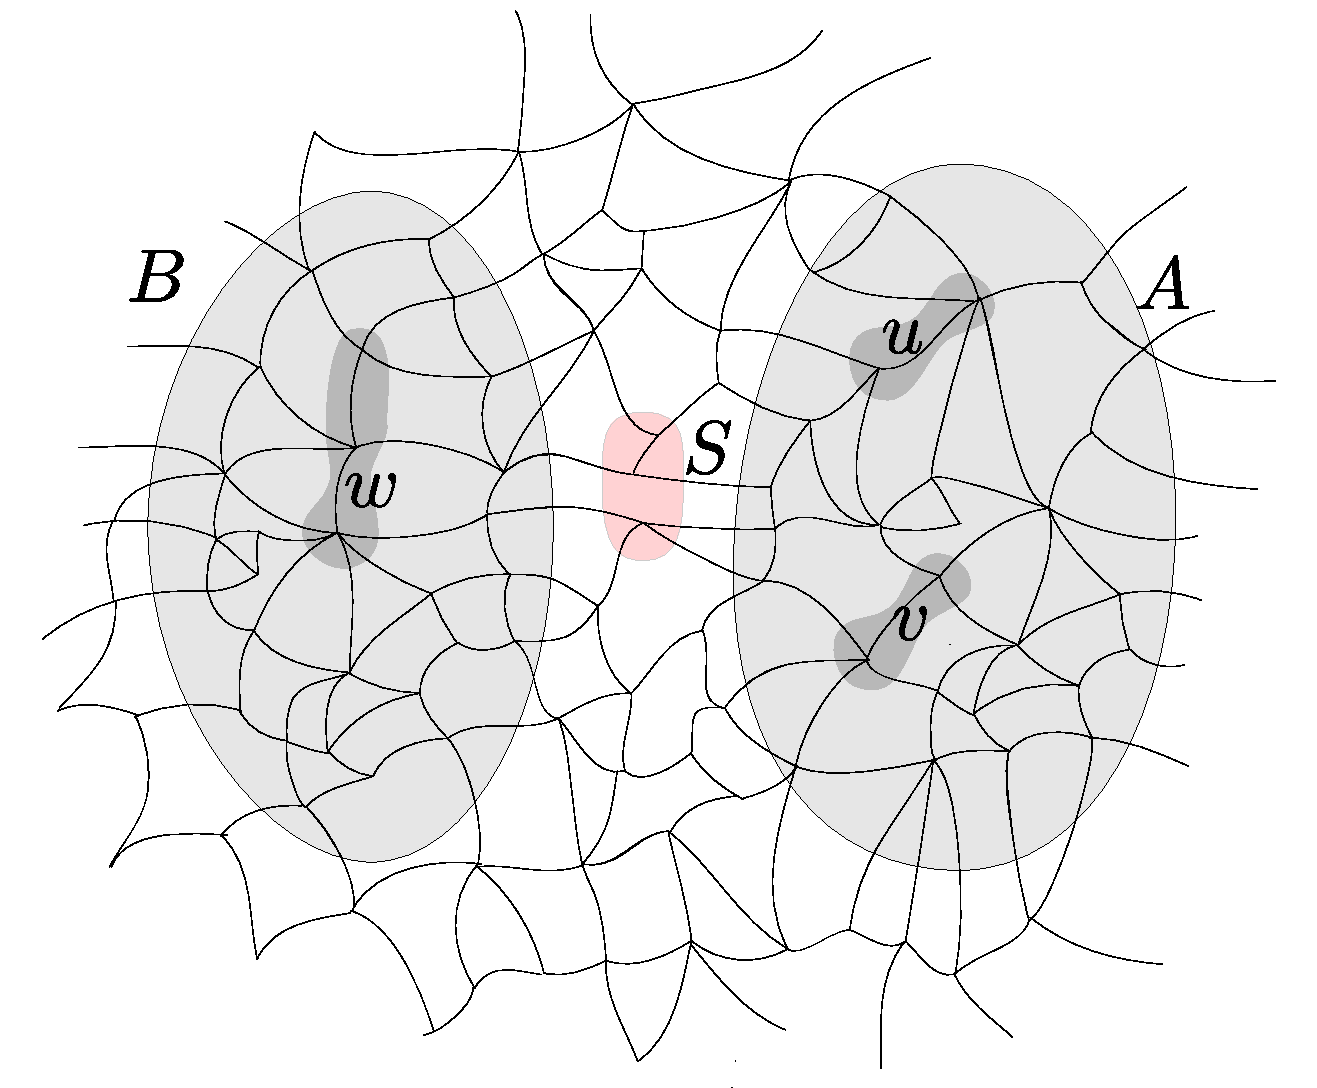
\includegraphics[scale=0.35,page=1]{pics}
 	\caption{The sets $A$ and $B$ are $2$-separated by $S$.
 	}
 	\label{fig:sep}
 \end{figure}
We remark that taking $r=\infty$ in $r$-separation yields the familiar notion of separation in graph theory,
and on the other hand, characterizes \emph{forking independence} in superflat graphs~\cite{ivanov}. Therefore,
$r$-separation can be thought of as a local analogue of forking independence, for nowhere dense graph classes.

A key lemma concerning $r$-separation (cf.~\cref{cor:bound}) states that if $A$
and $B$ are $r$-separated by a set $S$ of size $s$,
then for any fixed formula $\phi(\bar x,\bar y)$,
the set  $\{\{\tup b\ \in B^{|\bar x|} : \strA\models\phi(\tup a,\tup b)\} : \tup a\in A^{|\bar y|}\}$ has cardinality bounded by a constant depending on $s$ and $\phi$ only (and not on $G,A,$ and $B$). This elementary result combines  Gaifman's locality property and a Feferman-Vaught lemma. This, in combination with the polynomial bounds 
for uniform quasi-wideness (\cref{thm:new-uqw}, and its extension to tuples~\cref{thm:uqw-tuples}), as well as the previous results on neighborhood complexity~\cite{eickmeyer2016neighborhood,DrangeDFKLPPRVS16} are the main ingredients of our main result,~\cref{thm:vc-density}.

%
% \paragraph{Stability.}
%
%
% The second topic of study is the
% connection between nowhere denseness and stability theory.
% Fix
% % Let $\cal C$ be a class of structures over
%  a relational vocabulary $\Sigma$. Let
% $\phi(\tup{x},\tup{y})$ be a $\Sigma$-formula with the free variables
% partitioned into two groups $\tup{x}, \tup{y}$. A \emph{$\phi$-ladder}
% of length $n$ in a $\Sigma$-structure $\str A$ is a sequence $\tup{a}_1,\ldots, \tup{a}_{n},
% \tup{b}_1,\ldots, \tup{b}_{n}$ of tuples of elements of $\str A$
% such that for all $1\leq i,j\le n$,
% \[\strA\models\phi(\tup{a}_i,\tup{b}_j)\Longleftrightarrow i\leq j. \]
% The least  $n$ for which
% there is no $\phi$-ladder of length $n$ is
% the \emph{ladder index}
% of $\phi(\tup{x},\tup{y})$ in $\str A$ (which may depend on the way we split the
% variables). A class of graphs $\CCC$ is \emph{stable} if
% the ladder index of every first order formula $\phi(\tup{x},\tup{y})$ over
% graphs from $\CCC$ is bounded by a constant depending only on $\phi$
% and~$\CCC$.
%
% Podewski and Ziegler~\cite{podewski1978stable}
% consider \emph{superflat graphs}, a notion corresponding to uniform quasi-wideness in the
% infinite. They show that flat graphs are stable using an
% infinite Ramsey argument and compactness. Based on the
% results of Podewski and Ziegler,
% Adler and Adler~\cite{adler2014interpreting}
% proved that every nowhere dense class is stable, in fact, they
% proved that for a subgraph-closed class $\CCC$, the notions of
% nowhere denseness and stability coincide.
% However, their inherently non-constructive approach cannot give explicit upper bounds on parameters governing the stability of $\CCC$, for instance, the ladder indices.
%
% Based on the approach of Podewski and Ziegler~\cite{podewski1978stable}, we give a combinatorial
% proof that every first order formula has finite ladder index on every
% nowhere dense class, which does not involve infinite combinatorics and model theory.
% In particular, instead of compactness we use Gaifman's Locality Theorem for
% first order logic~\cite{gaifman1982local}. The following theorem summarizes our~result.
%
% \begin{theorem}\label{thm:new-stable}
%   There are computable functions $f\colon \N^3\to\N$ and $g\colon\N\to\N$ with the following property.
% Suppose $\phi(\bar x,\bar y)$ is a formula of quantifier rank $q$ and with $d$ free variables,
% and $G$ is a graph such that $K_t\not\minor_{g(q)} G$. Then the ladder index of $\phi(\bar x,\bar y)$ in $G$ is at most $f(q,d,t)$.
% \end{theorem}
%
% Note that in particular, \cref{thm:new-stable} implies that every nowhere dense graph is stable, which was the main conclusion of Adler and Adler~\cite{adler2014interpreting}.
%
% We remark that the above connections between nowhere denseness and notions from model theory have recently found algorithmic applications.
% Both uniform quasi-wideness and stability techniques are key tools used in the study of the complexity of the {\sc Distance-$r$ Dominating Set} problem on nowhere dense graph classes,
% and in particular in the design of polynomial kernelization procedures for this problem~\cite{DawarK09,drange2016kernelization,eickmeyer2016neighborhood,siebertz2016polynomial}.


\paragraph{Organization.} In \cref{sec:uqw} we recall standard concepts from the theory of sparse graphs and prove \cref{thm:new-uqw}, improving greatly the previously the previous bounds.
In~\cref{sec:uqw-tuples} we formulate and prove the  generalization to tuples,~\cref{thm:uqw-tuples}. This result is new in the context of nowhere dense graph classes, and is an important tool for the further results.
In \cref{sec:gaifman} we discuss Gaifman locality for first order logic and derive an elementary variant  concerning local separators.
 In \cref{sec:types} we prove our main result, \cref{thm:vc-density}, and of the corresponding lower bounds, given by \cref{thm:vc-density-lower-bound}.
Finally, in \cref{sec:stable} we provide an effective proof of the result of Adler and Adler, \cref{thm:new-stable}.

%\end{change}

%\pagebreak


% Finally, we observe that an argument of Bousquet and
% Thomasse\'e~\cite{BousquetT15} can be slightly modified to prove that
% the VC-dimension of the $r$th power $G^r$ of a graph $G$
% with $K_t\not\minor_r G$ is bounded by $t-1$.
% Boundedness of VC-dimension is a weaker condition than the stability of a class, however it is sufficient in many contexts.
% Therefore, we consider investigating explicit bounds on the VC-dimension potentially useful for future research.
%
% \begin{theorem}\label{thm:new-vc}
% Let $G$ be a graph such that $K_t\not\minor_r G$. Then the
% VC-dimension of $G^r$, the $r$th power of the graph~$G$, is bounded by $t-1$.
% \end{theorem}

%\paragraph{Organization.} We give background from graph theory in \cref{sec:uqw}, where we also
%prove \cref{thm:new-uqw}. 
%We provide background 
%on logic and prove \cref{thm:new-stable} in \cref{sec:stable}. 



